\chapter{Хэрэгжүүлэлт}

Энэхүү бүлэгт өмнө нь гарсан интерфэйс дизайн, системийн архитектур болон диаграмуудыг хэрэгжүүлж хэрхэн бүтээгдэхүүн болгон гаргасан талаараа бичлээ. Хэрэгжүүлэлт хийх үе шатаа ерөнхийд нь

\begin{itemize}
	\item Хөгжүүлэлтийн орчноо бэлдэх
	\item Front-end болон Back-end хөгжүүлэлт
	\item Серверт байршуулах /Deploy/
\end{itemize}

гэсэн алхмуудад хувааж гүйцэтгэсэн ба доор ажлуудаасаа гол гэсэн зүйлсээ нэгтгэн оруулав.

\section{Хөгжүүлэлтийн орчныг бэлдэх}
\label{section:backend}

Ашиглах технологийн хувьд Next.js, Prisma ORM, PostgreSQL ашиглах учир хамгийн эхлээд өгөгдлийн сангаа Local хост дээрээ бэлдэж, дараа нь Next.js фрэймворкоо суулган шаардлагатай тохиргоонуудыг хийнэ. Үүний дараагаас Prisma ORM-ээ суулгаж, урьдчилж бэлдсэн Next.js төсөл дээрээ орууллаа. 

Мөн кодын хувилбараа хадгалж, хөгжүүлэлтийн үе шатаа цэгцтэй авч явахын тулд  Version Control дээрээ Git, Github.com-г сонгож private харагдацтай repository үүсгэв. 

\clearpage
\begin{figure}[h]
	\centering
	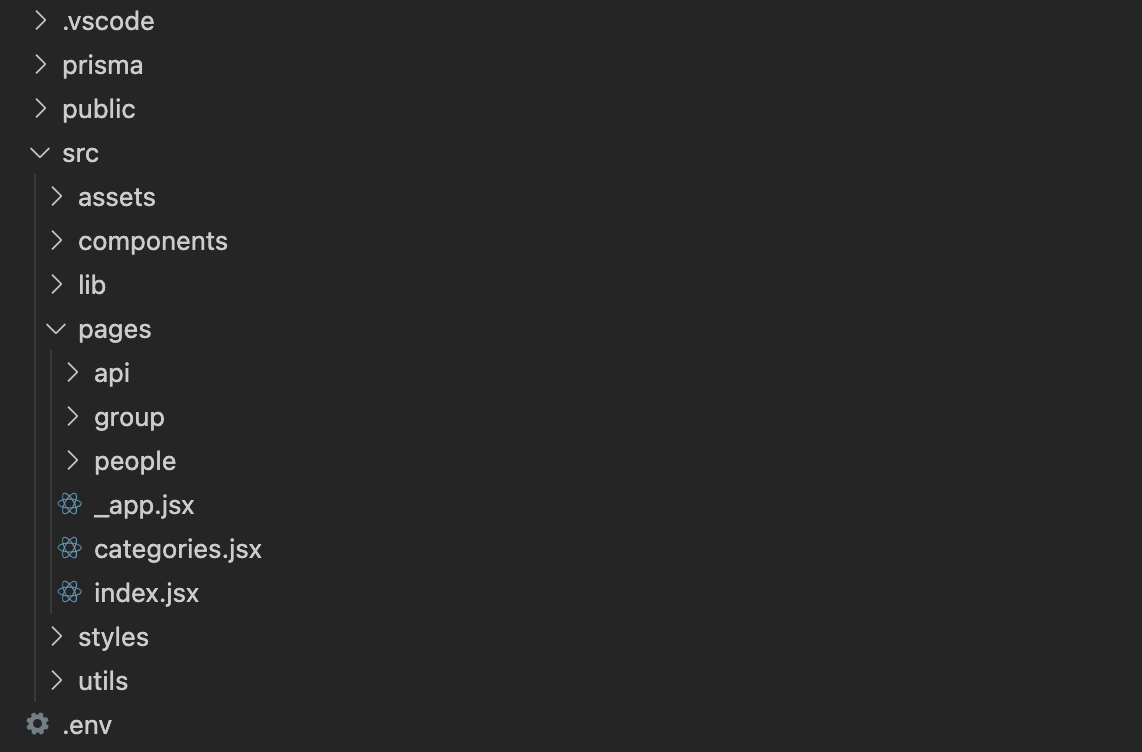
\includegraphics[width=10cm]{images/implement/file-structure.png}
	\caption{Төслийн файлын бүтэц}
	\label{fig:file-structure}
\end{figure}

Next.js дээр файлын бүтцээ Зураг 4.1 дээр харагдаж байгаачлан бүтэцлэж хөгжүүлэлтээ эхлэхэд бэлэн болголоо. Хөгжүүлэлтийн гол зорилго маань Fullstack хөгжүүлэлт хийх учир манай платформын back-end, front-end хэсгүүд нэг repository дотор хамт явагдана. Файлын бүтцээ тайлбарлавал

\begin{itemize}
	\item \textbf{prisma} хавтаст цаашдаа ашиглах моделууд бичигдсэн schema байршина
	\item \textbf{public} хавтаст төслийн хүрээнд ашиглах статик файлууд /зураг, icon/ байна
	\item \textbf{src} хавтаст төслийн бүх компонент, гол эх кодууд байршина
	\item \textbf{src/pages/api} хавтаст төслийн back-end хэсгийн код бичигдэнэ
\end{itemize}

\section{Код хөгжүүлэлт}

Хөгжүүлэлтийн хувьд маш олон компонент, хуудсууд, тэдгээрийн код хийгдсэн тул зөвхөн нүүр хуудас буюу хэрэглэгчийн дагаж буй хүмүүсийн оруулсан холбоосууд харагддаг хэсгийг онцолж авч эхнээс нь эхлээд бүтэн ажиллах үе шатуудыг тайлбарлав.

\subsection{Гаргасан интерфэйсийнхээ дагуу хэрэглэгчид харагдах хэсгийг өрсөн нь}

Front-end хөгжүүлэлт дээр урьдчилж интерфэйс дизайныг гаргасан нь вебийн бүх компонент, тэдгээр хаана байрших гээд олон зүйлийг тодорхой болгож өгсөн нь давуу тал болж өгсөн. Иймд хамгийн эхлээд бэлдсэн хөгжүүлэлтийн орчин дээрээ үндсэн хуудсууд болон дотор нь ашиглаж буй компонентуудыг статик байдлаар өрөв. 

\begin{lstlisting}[language=Javascript, caption=Хэрэглэгчийн оруулсан холбоосыг харагдах компонент, frame=single]
	export const Card = ({
  href,
  type,
  site_url,
  og_title,
  og_image,
  author_name,
  author_profile,
  vote_count,
  tags,
}) => {
  return (
    <Link href={href} target="_blank">
      <div className="cursor-pointer space-y-2 rounded-lg border border-gray200 bg-gray300 p-3.5 transition-all duration-300 hover:border-gray100 hover:bg-white hover:shadow-sm">
        <div className="flex items-center gap-1 text-sm font-normal text-description">
          <LinkIcon />
          {site_url}
        </div>
	       
					...

          <div className="order-last flex items-center gap-1 text-sm text-description">
            <VoteBtn type="up" />
            <VoteBtn type="down" />
          </div>
        </div>
      </div>
    </Link>
  );
};
			
\end{lstlisting}


\subsection{Prisma ORM ашиглаж өгөгдлийн сангаа бэлдэх}

Хамгийн түрүүнд өгөгдлийн сангийн схемийнхээ дагуу \textbf{prisma/schema.prisma} файл дээр өгөгдлийн сан дээр үүсгэх хүснэгт, багануудын бүх нөхцөл, холбоосуудыг бичиж хэрэглэгчийн оруулсан нийтлэлийн өгөгдлийг хадгалах \textbf{Post} гэсэн хүснэгтийг үүсгэнэ.

\begin{lstlisting}[language=Javascript, caption=Өгөгдлийн сангийн хүснэгтийг Prisma ашиглан үүсгэх, frame=single]
	generator client {
		provider = "prisma-client-js"
	}
	
	datasource db {
		provider = "postgresql"
		url      = env("DATABASE_URL")
	}
	
	model Post {
		id       Int    @id @default(autoincrement())
		siteUrl  String
		ogTitle  String
		ogImage  String
		authorId Int
		author   User   @relation(fields: [authorId], references: [id], onDelete: Cascade)
		groupId  Int?
		group    Group? @relation(fields: [groupId], references: [id])
		tags       Tag[]
		categories Category[]
		createdAt DateTime @default(now())
		updatedAt DateTime @updatedAt
	}	

	...

\end{lstlisting}

Уг файлыг \textbf{migration} хийсний дараа бичсэн моделийн дагуу өгөгдлийн сан дээр \textbf{Post} хүснэгт үүссэн. 

\begin{figure}[h]
	\centering
	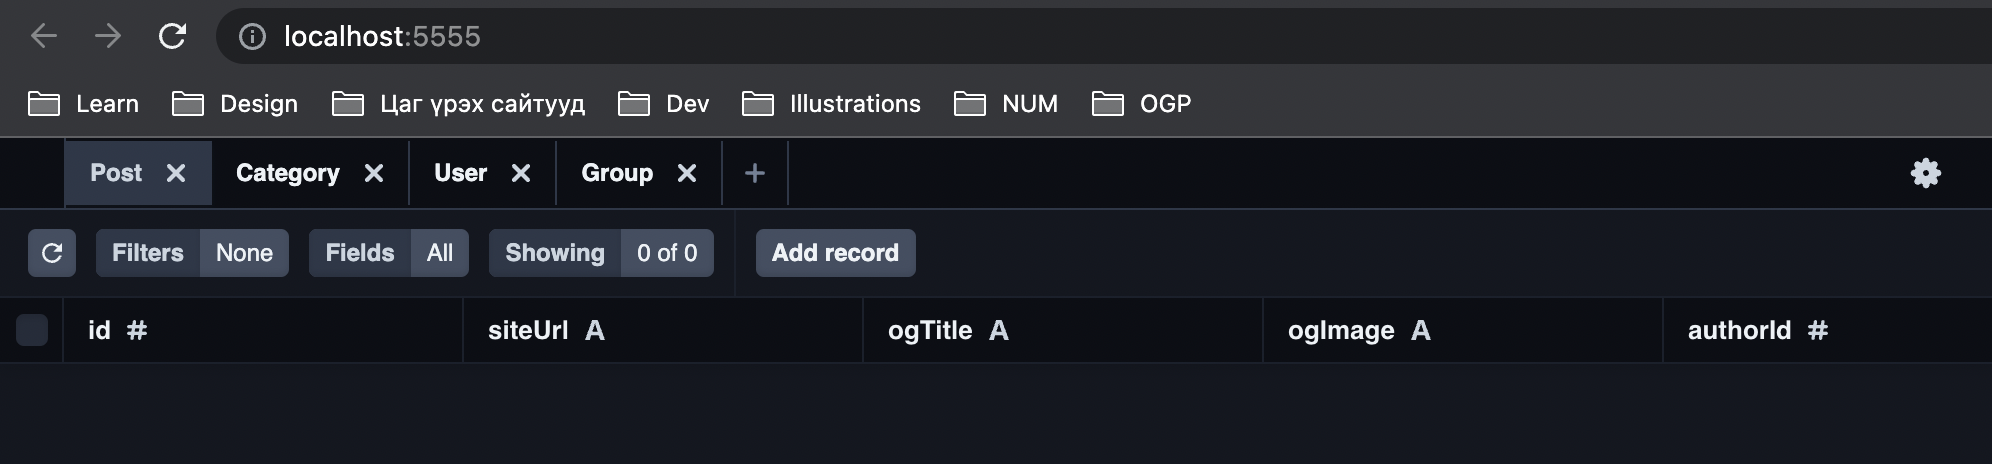
\includegraphics[width=10cm]{images/implement/table.png}
	\caption{Post хүснэгтийн харагдац}
	\label{fig:table}
\end{figure}

\subsection{Хэрэглэгчийн оруулсан холбоосын жагсаалтыг харах End point гаргах}

Back-end хэсгийн кодыг түрүүн хэлсэнчлэн шууд Next.js фрэймворк дээрээ \textbf{/api/posts/index.js} гэсэн файл үүсгэж Prisma Client сангаас шаардлагад нийцсэн функцүүдийг хэрэглэж хэрэгтэй өгөгдлийг тодорхой нөхцлүүдээр авч хариуг буцаана.

\begin{lstlisting}[language=Javascript, caption=Next.js дээрээ end point гаргах, frame=single]
	import prisma from "../../../lib/prisma";

export default async function handle(req: NextApiRequest, res: NextApiResponse) {
    const requestMethod = req.method
    switch (requestMethod){
        case 'GET':
            let following;
            try{
                following = await getFollowing(1)
                console.log(following)
            } catch (e) {
                if (e instanceof Prisma.PrismaClientKnownRequestError) {
                    if (e.code === 'P2002') {
                        res.json([])
                    } else{
                        res.status(400).json(e)
                    }
                } else {
                    console.log(e)
                    res.status(500).json({message: "something wrong try again some time later"})
                }
            }

            try {
                const posts = await getPostsByUsers(following.map(follow=>{
                return follow.following
            }))
                
            const curPosts = posts.map(p => {
                return {
                    id: p.id,
                    ogImage: p.ogImage,
                    ogTitle: p.ogTitle,
                    ogUrl: p.ogUrl,
                    groupId: p.groupId,
                    group: p.group,
                    tags: p.tags,
                    authorId: p.authorId,
                    author: p.author,
                    categories: p.categories[0].id || ''
                }
            })                

            res.json({list:curPosts,total:posts.length})

            } catch (e) {
                if (e instanceof Prisma.PrismaClientKnownRequestError) {
                    if (e.code === 'P2002') {
                        res.json({list:[],total:0})
                    }else{
                        res.status(400).json(e)
                    }
                } else {
                    console.log(e)
                    res.status(500).json({message: "something wrong try again some time later"})
                }
            }
            break
        default: res.status(404)
    }
}

...

\end{lstlisting}

Уг кодны үр дүнд дараах JSON object үүссэнийг Postman ашиглаж GET хүсэлт тавин харууллаа.

\begin{figure}[h]
	\centering
	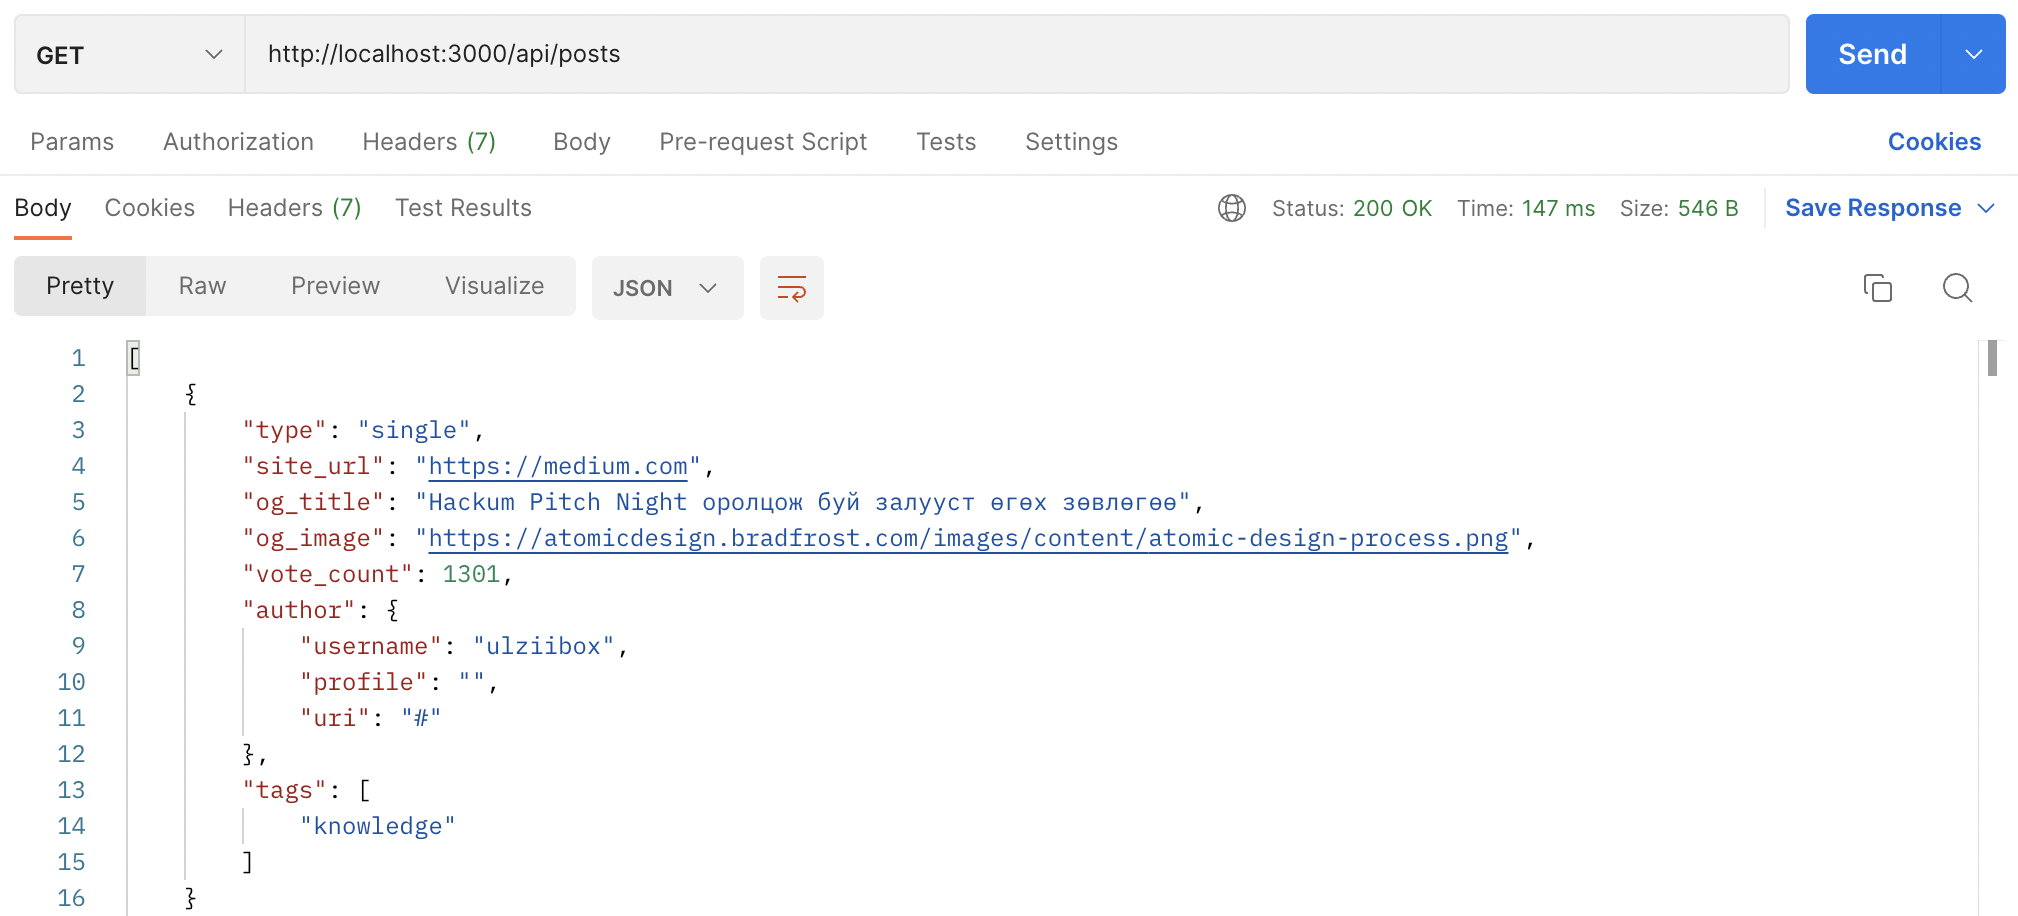
\includegraphics[width=13cm]{images/implement/endpoint.png}
	\caption{Нийтлэлийн жагсаалтыг агуулсан JSON Object}
	\label{fig:endpoint}
\end{figure}

\subsection{Front-end хэсэг дээр гаргасан End point-оо ашиглаж бодит өгөгдлийг харуулах}

Одоо Front-end хэсэг дээрээ нийтлэлийн жагсаалтуудыг авч нүүр хуудаст зурж харуулах шаардлагатай. Үүний тулд axios хүсэлтийг ашиглаж өгөгдлөө авч өмнө нь үүсгэсэн \textbf{Card} компонентдоо шаардлагатай \textbf{props}-уудыг дамжуулж, нийтлэлийг \textbf{map} функцийг ашиглан харуулав

\begin{lstlisting}[language=Javascript, caption=ServerSideProps болон axios ашиглан хүсэлт илгээж өгөгдлөө татаж авах, frame=single]
	
export async function getServerSideProps() {
	const { data: categories } = await axios.get(
		`${process.env.API_URL}/categories`
	);
	const { data: posts } = await axios.get(
		`${process.env.API_URL}/posts/following`
	);
  return {
    props: {
      categories: categories || [],
      posts: posts || [],
    },
  };
}

\end{lstlisting}

\begin{lstlisting}[language=Javascript, caption=Card компонентод ирсэн утгуудыг props-оор дамжуулж DOM дээр рендерлэх, frame=single]
	
	...
	const router = useRouter();

  useEffect(() => {
  
    setCategories([
      {
        id: 0,
        name: "Бүгд",
      },
      ...CATEGORIES,
    ]);
  }, []);

	... 

	{posts.map((item) => {
		if (item.type === "single") {
			return (
				<Card
					key={item.post.id}
					site_url={item.post.site_url}
					og_title={item.post.og_title}
					og_image={item.post.og_image}
					author_name={item.post.author.username}
					author_profile={item.post.author.profile_img}
					vote_count={item.post.vote_count}
					tags={item.post.tags}
					href={item.post.href}
				/>
			);
		}
	}}

	...

\end{lstlisting}

\section{Үр дүн}

Дээрх үйлдлүүд нь манай төслийг хэрхэн ажиллаж буйг тоймлон харуулсан ба үр дүнд нь хэрэглэгчийн дагаж буй хүмүүсийн оруулсан холбоосууд нүүр хуудас дээр харагдана. 

\begin{figure}[h]
	\centering
	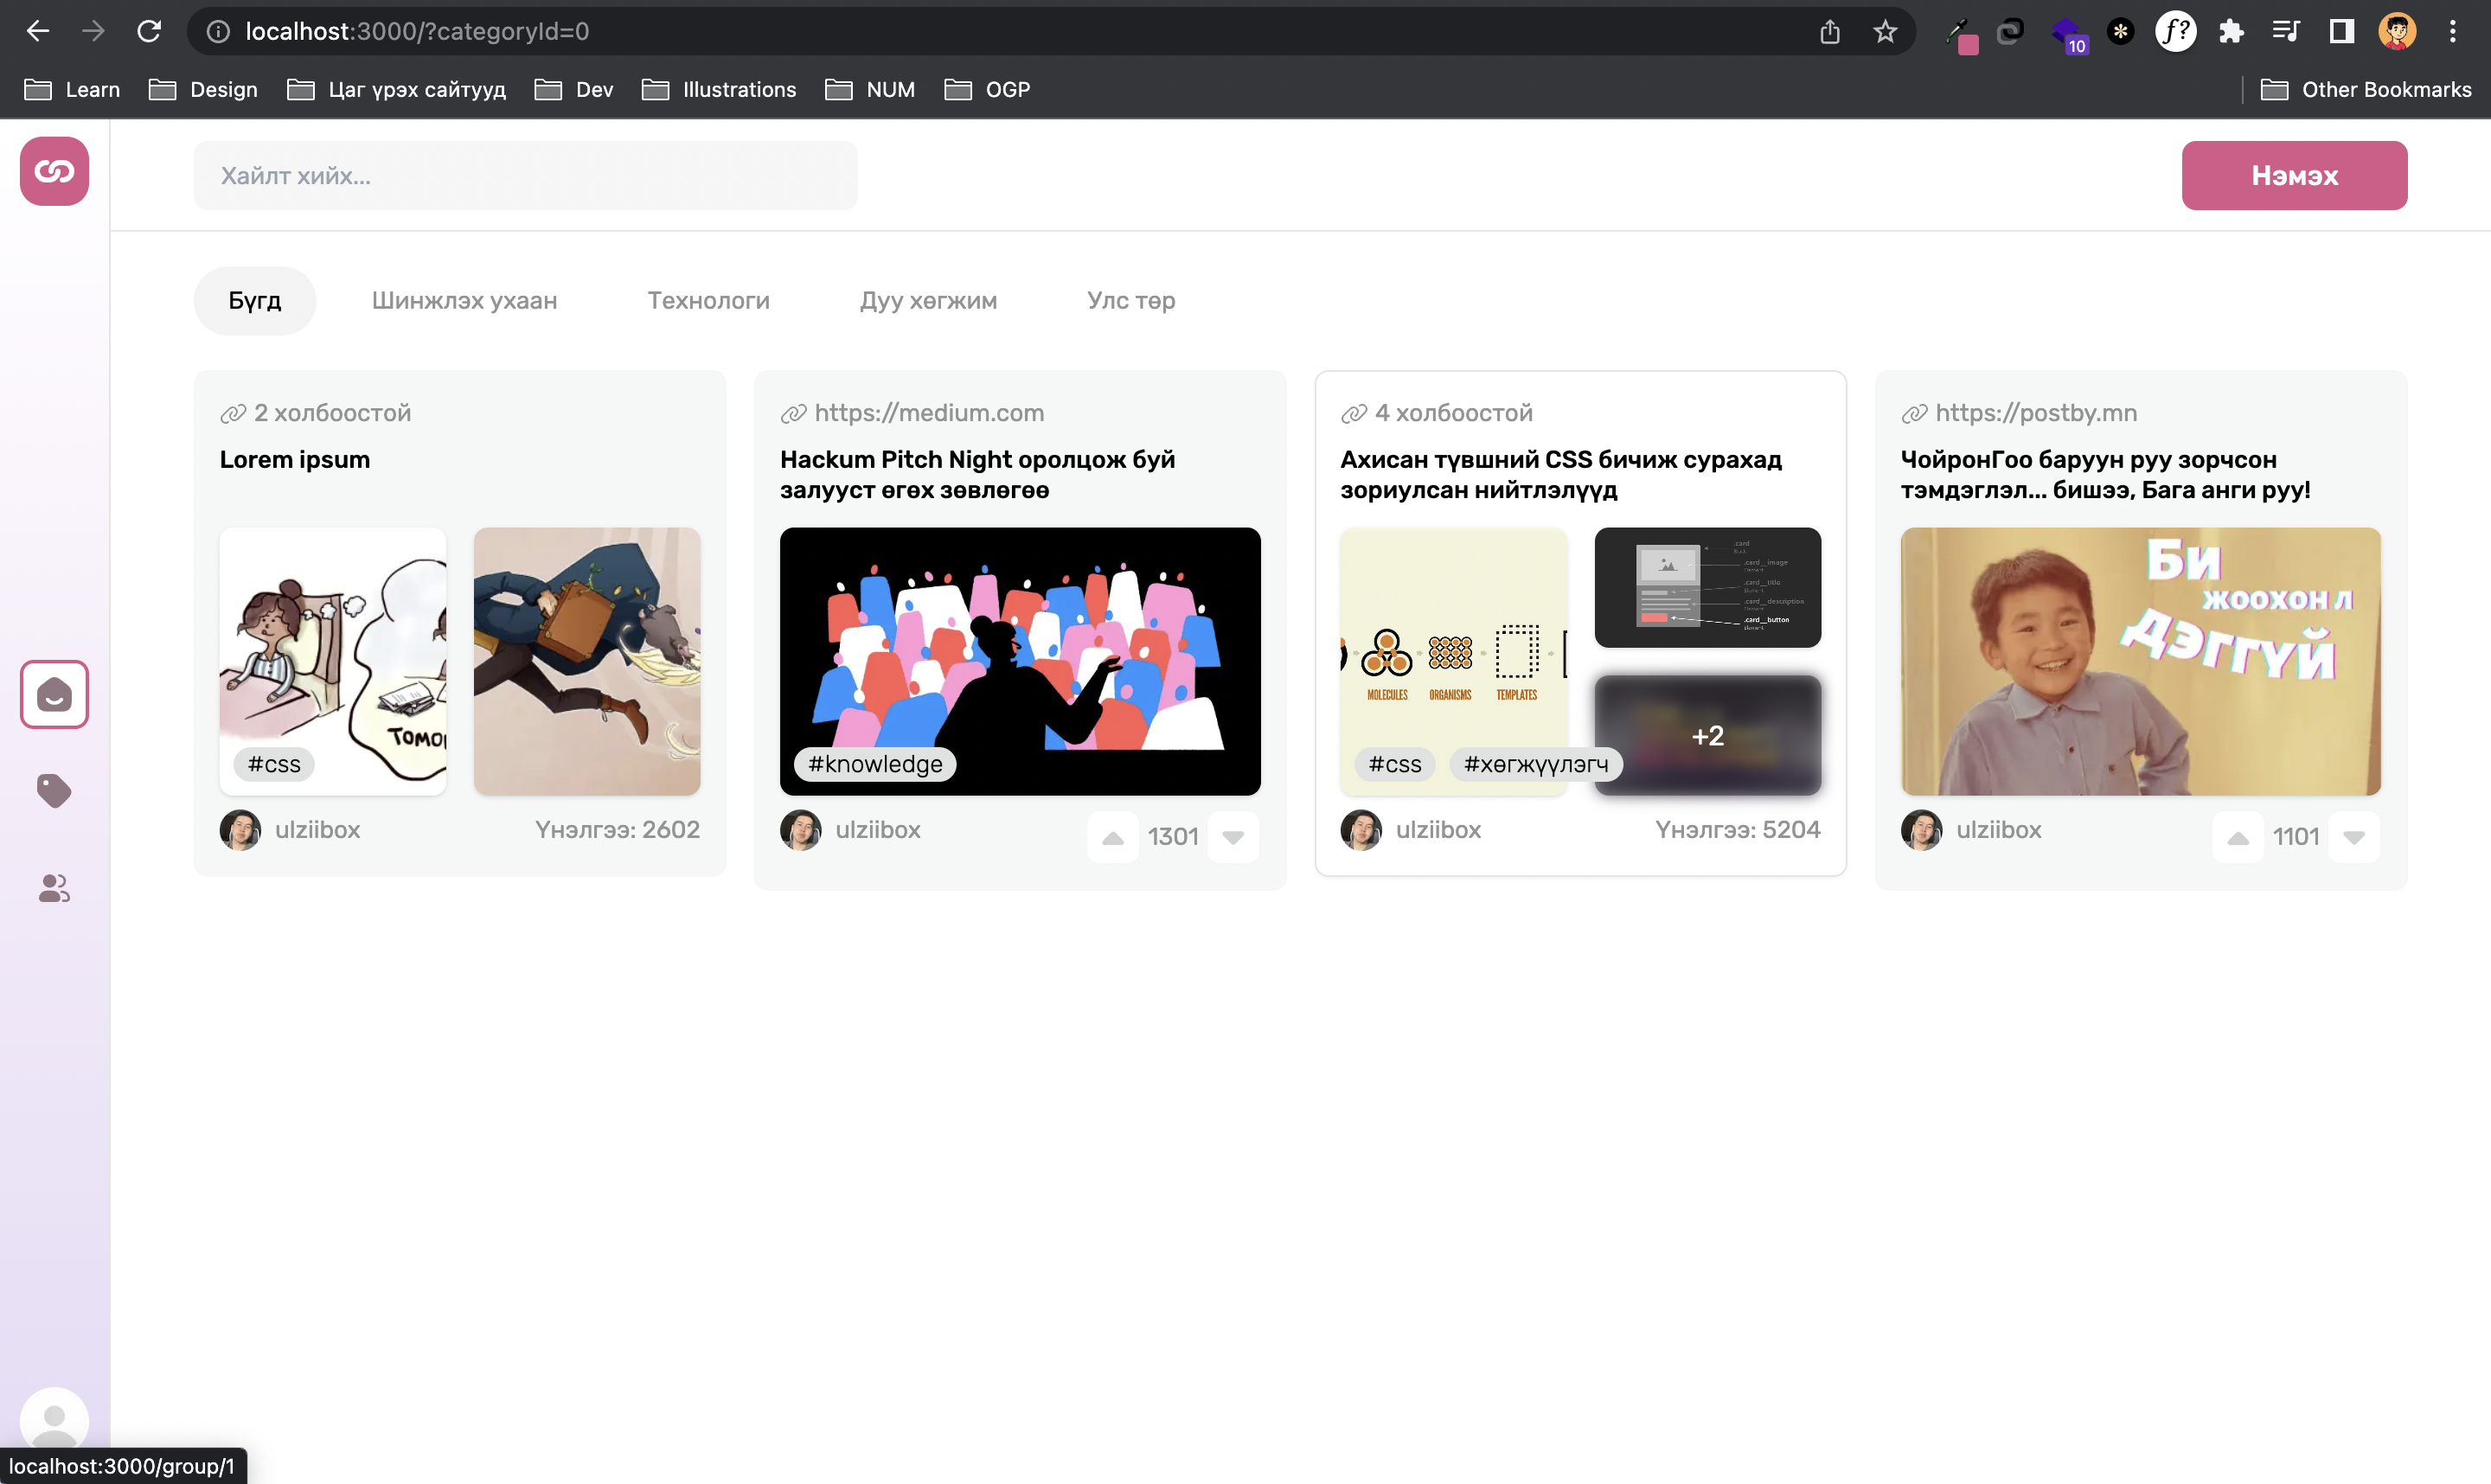
\includegraphics[width=13cm]{images/implement/home-page.png}
	\caption{Нүүр хуудас}
	\label{fig:home-page}
\end{figure}

Мөн цаашид дээрх байдлаар шаардлагын дагуу гарсан интерфэйсүүдийг хийж дуусгах ба платформынхоо зарим зургаас оруулав.

\begin{figure}[h]
	\centering
	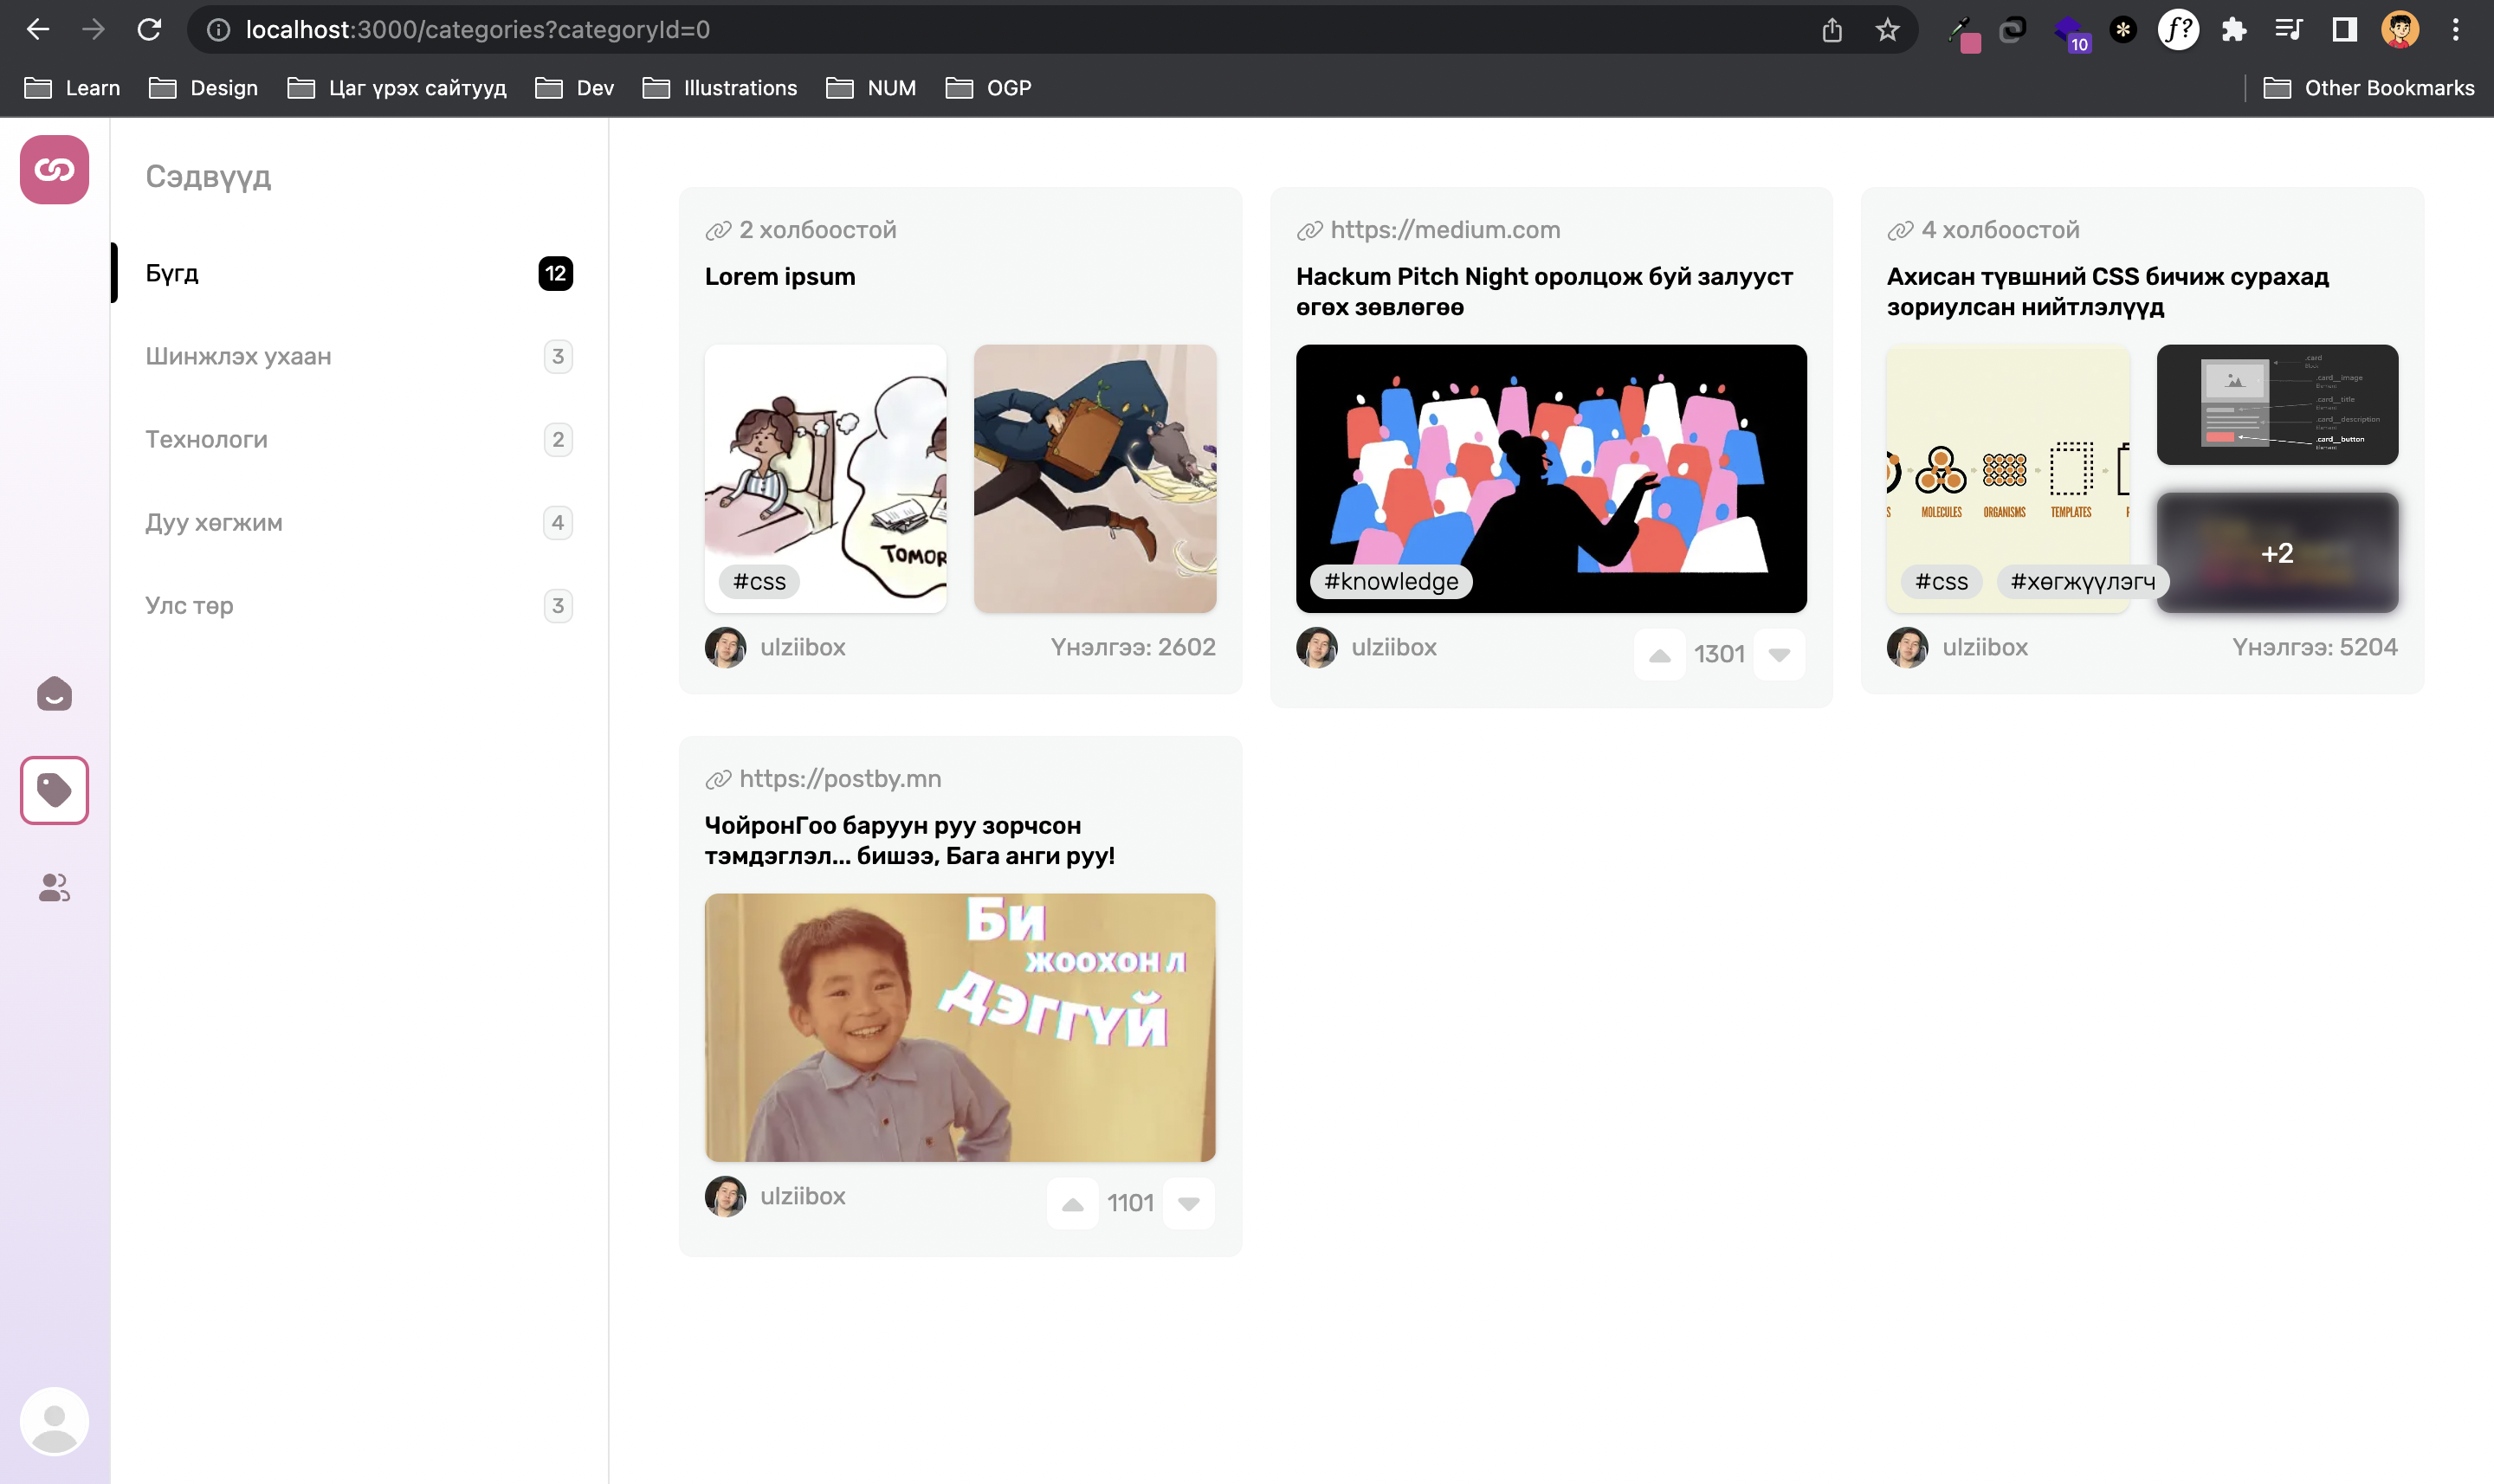
\includegraphics[width=13cm]{images/implement/category.png}
	\caption{Платформ дээрх сэдвүүдийн жагсаалт болон бүх нийтлэлийг харах}
	\label{fig:category}
\end{figure}

\begin{figure}[h]
	\centering
	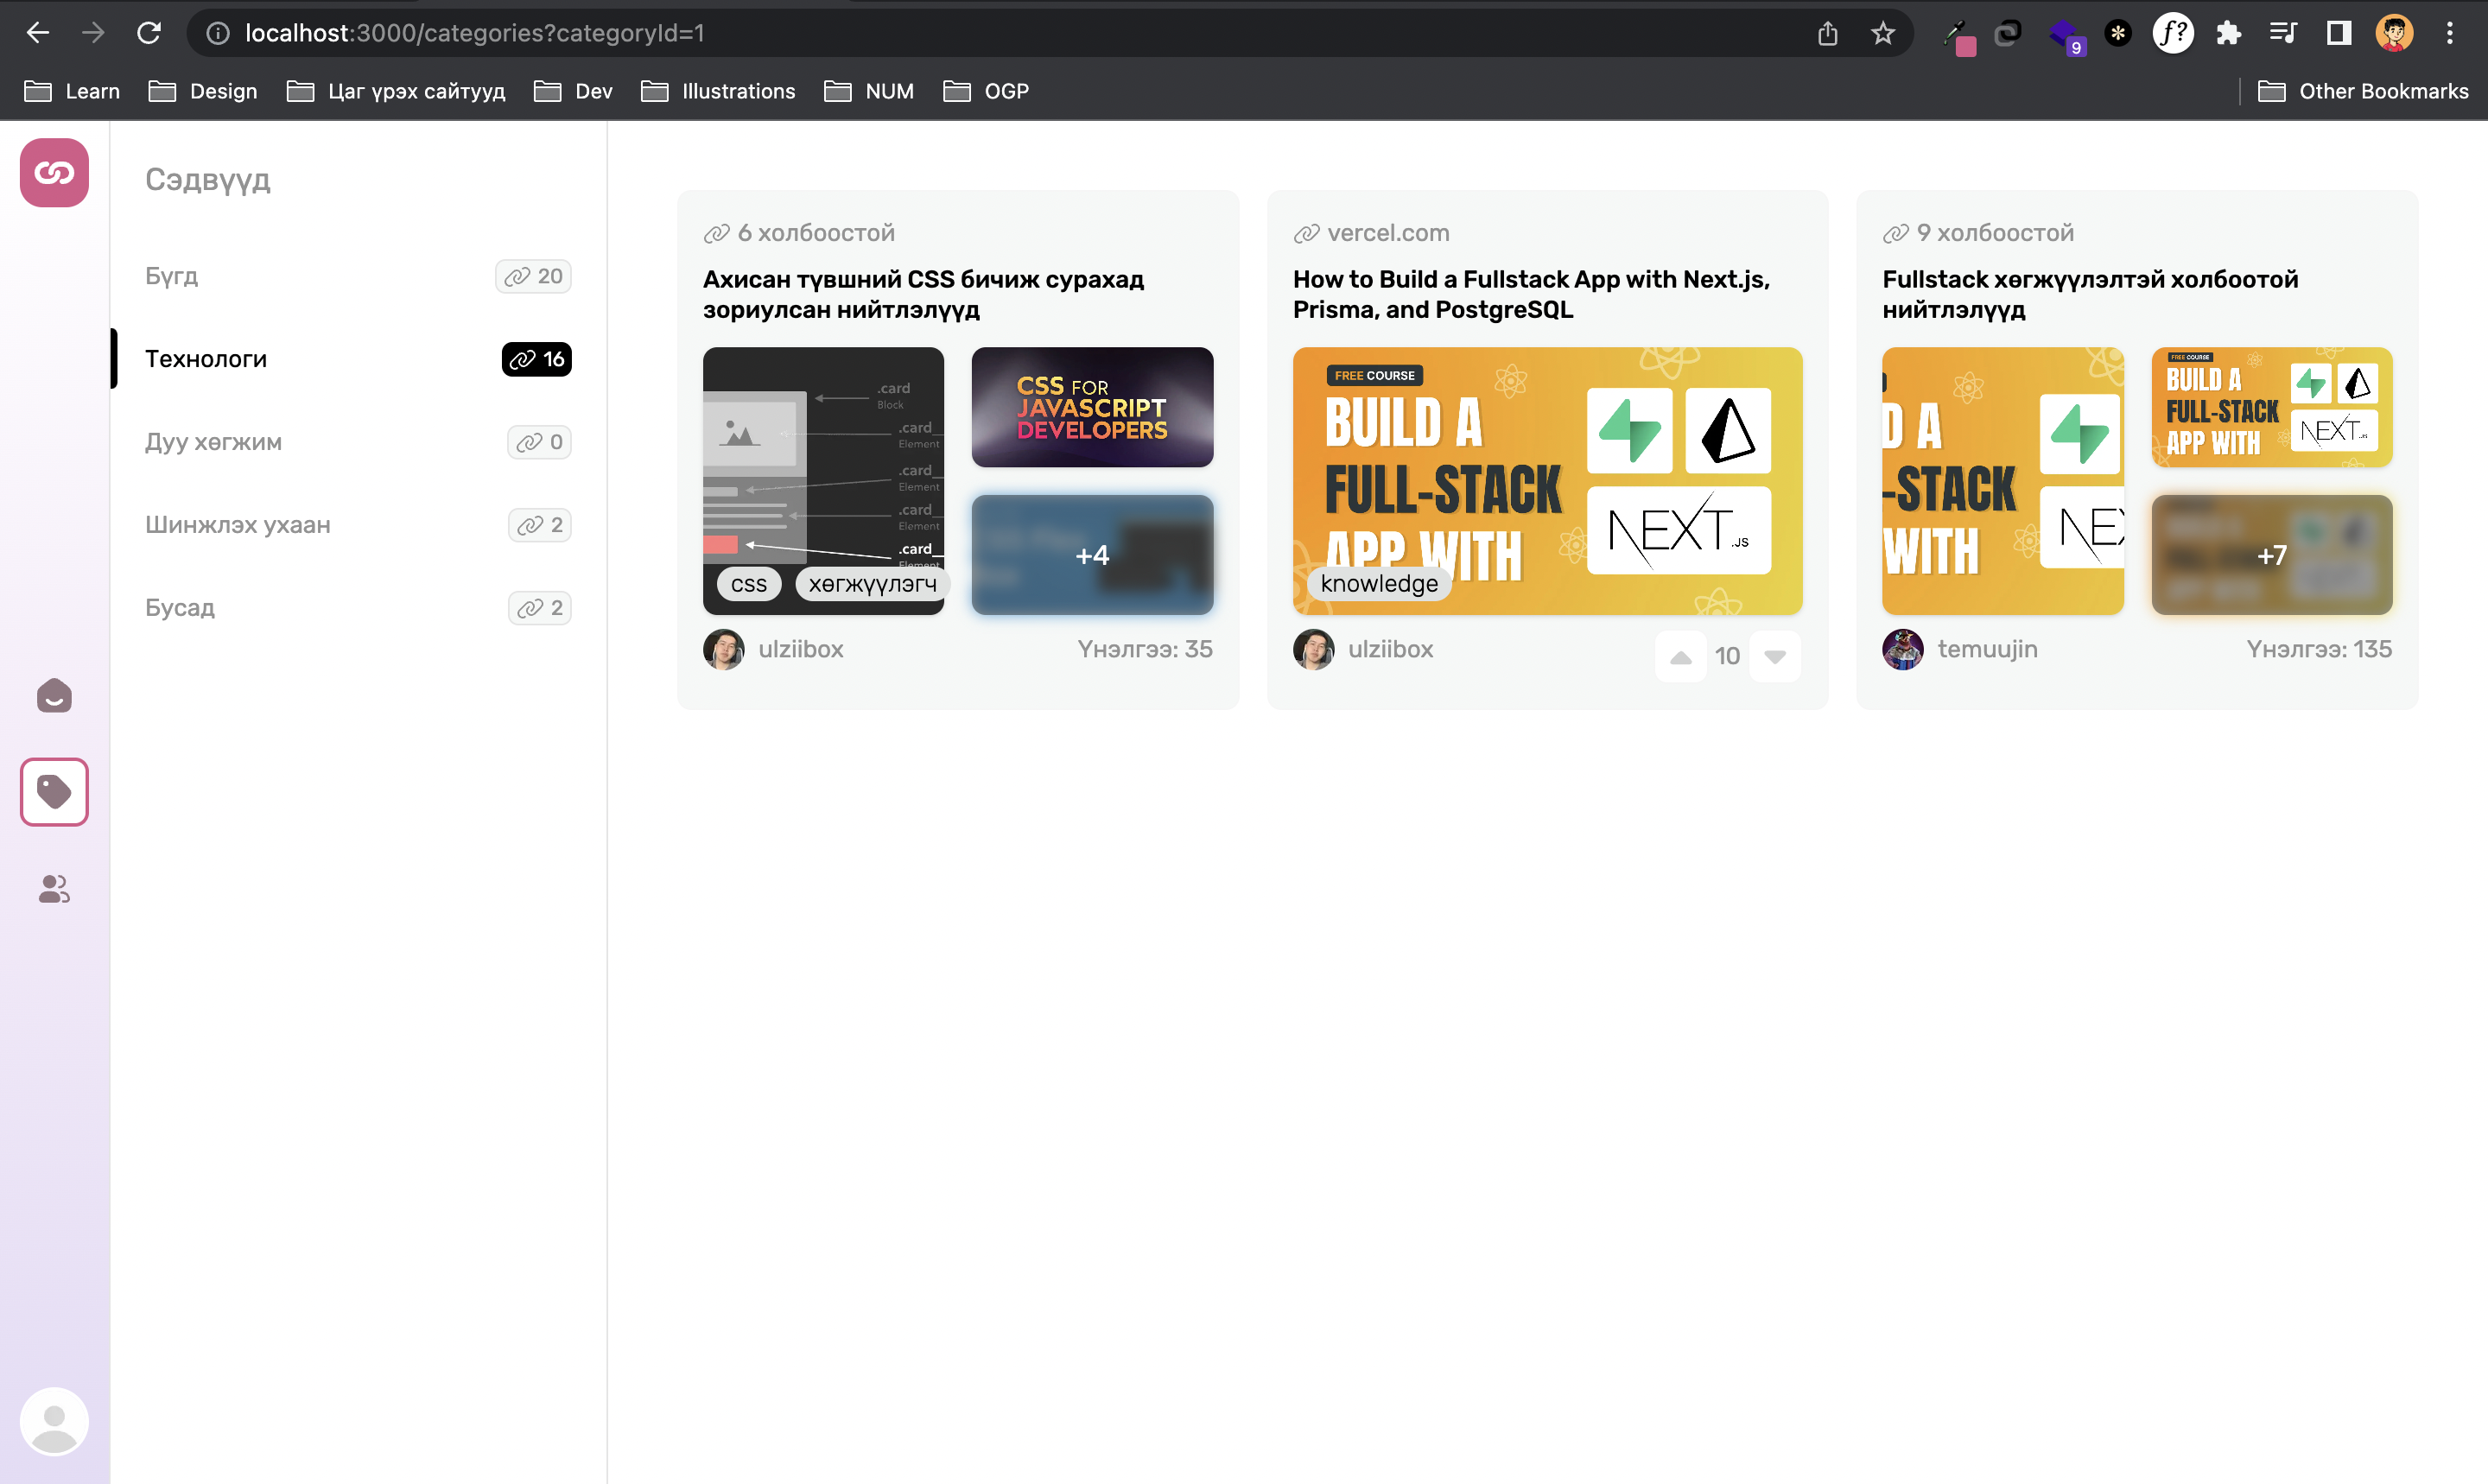
\includegraphics[width=13cm]{images/implement/category-filter.png}
	\caption{Холбоосуудыг сэдвээр нь шүүж харах}
	\label{fig:category-filter}
\end{figure}

\begin{figure}[h]
	\centering
	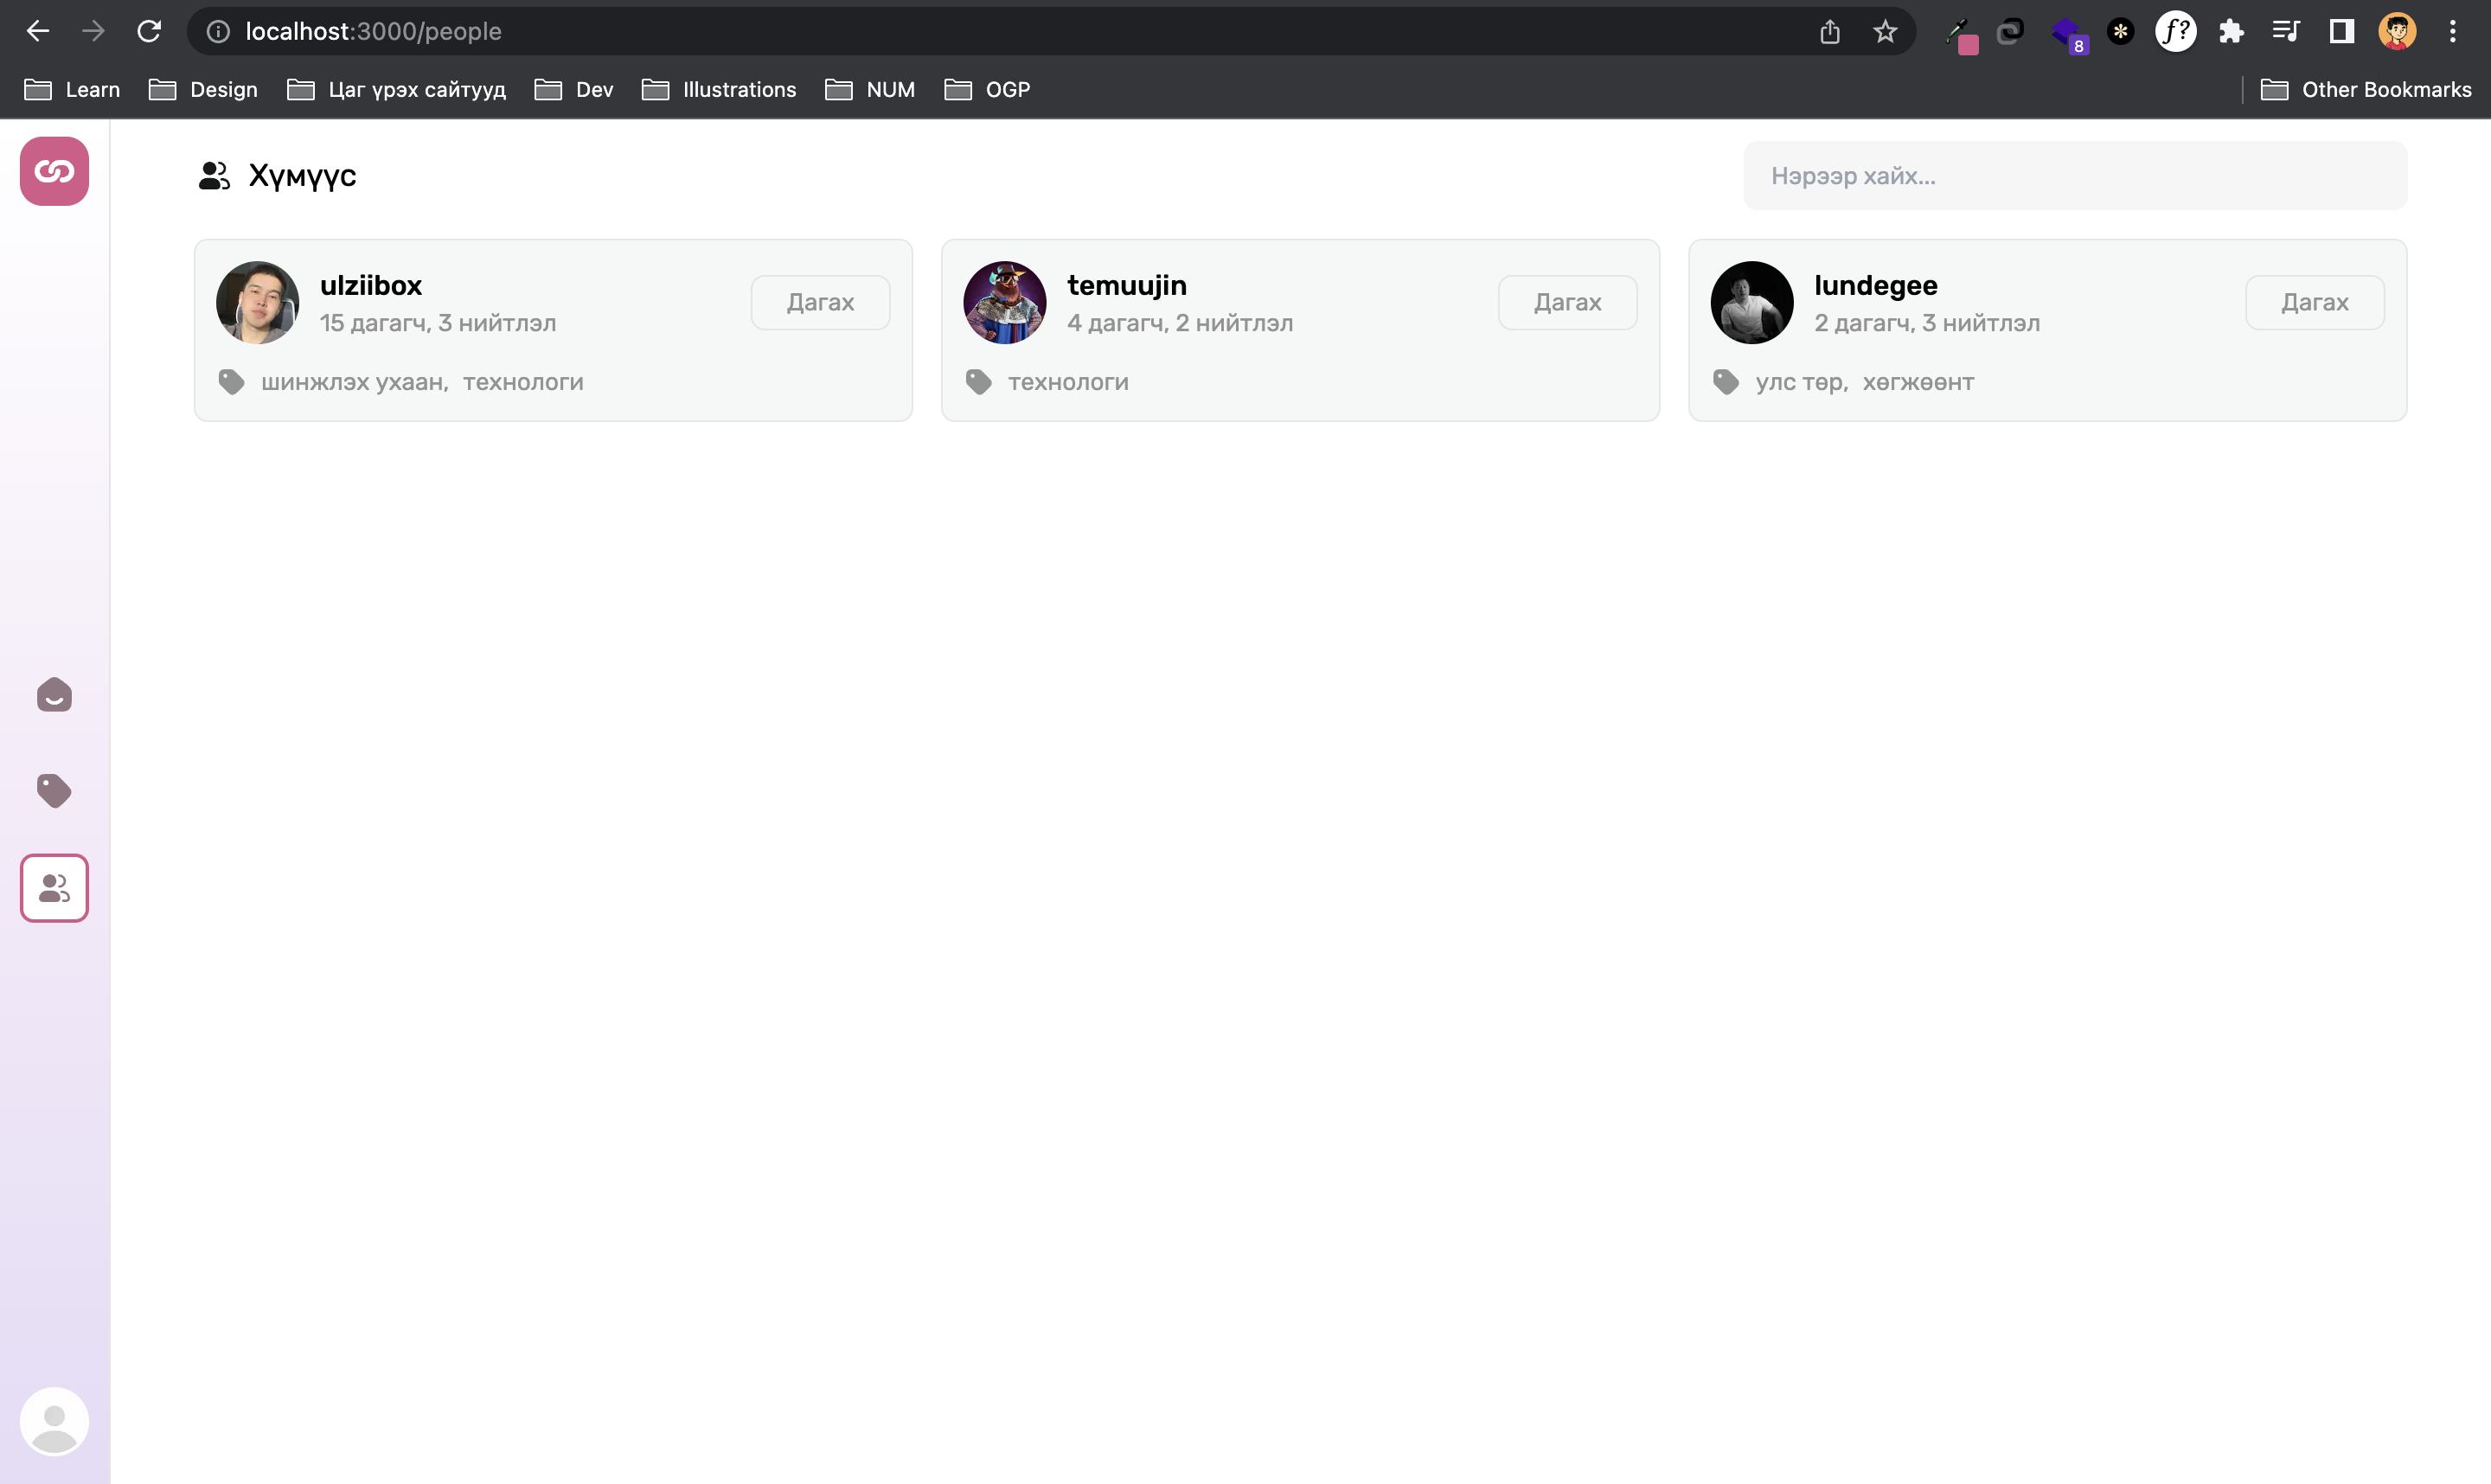
\includegraphics[width=13cm]{images/implement/users.png}
	\caption{Платформ дээр бүртгүүлсэн хэрэглэгчдийн жагсаалтыг харах}
	\label{fig:users}
\end{figure}

\begin{figure}[h]
	\centering
	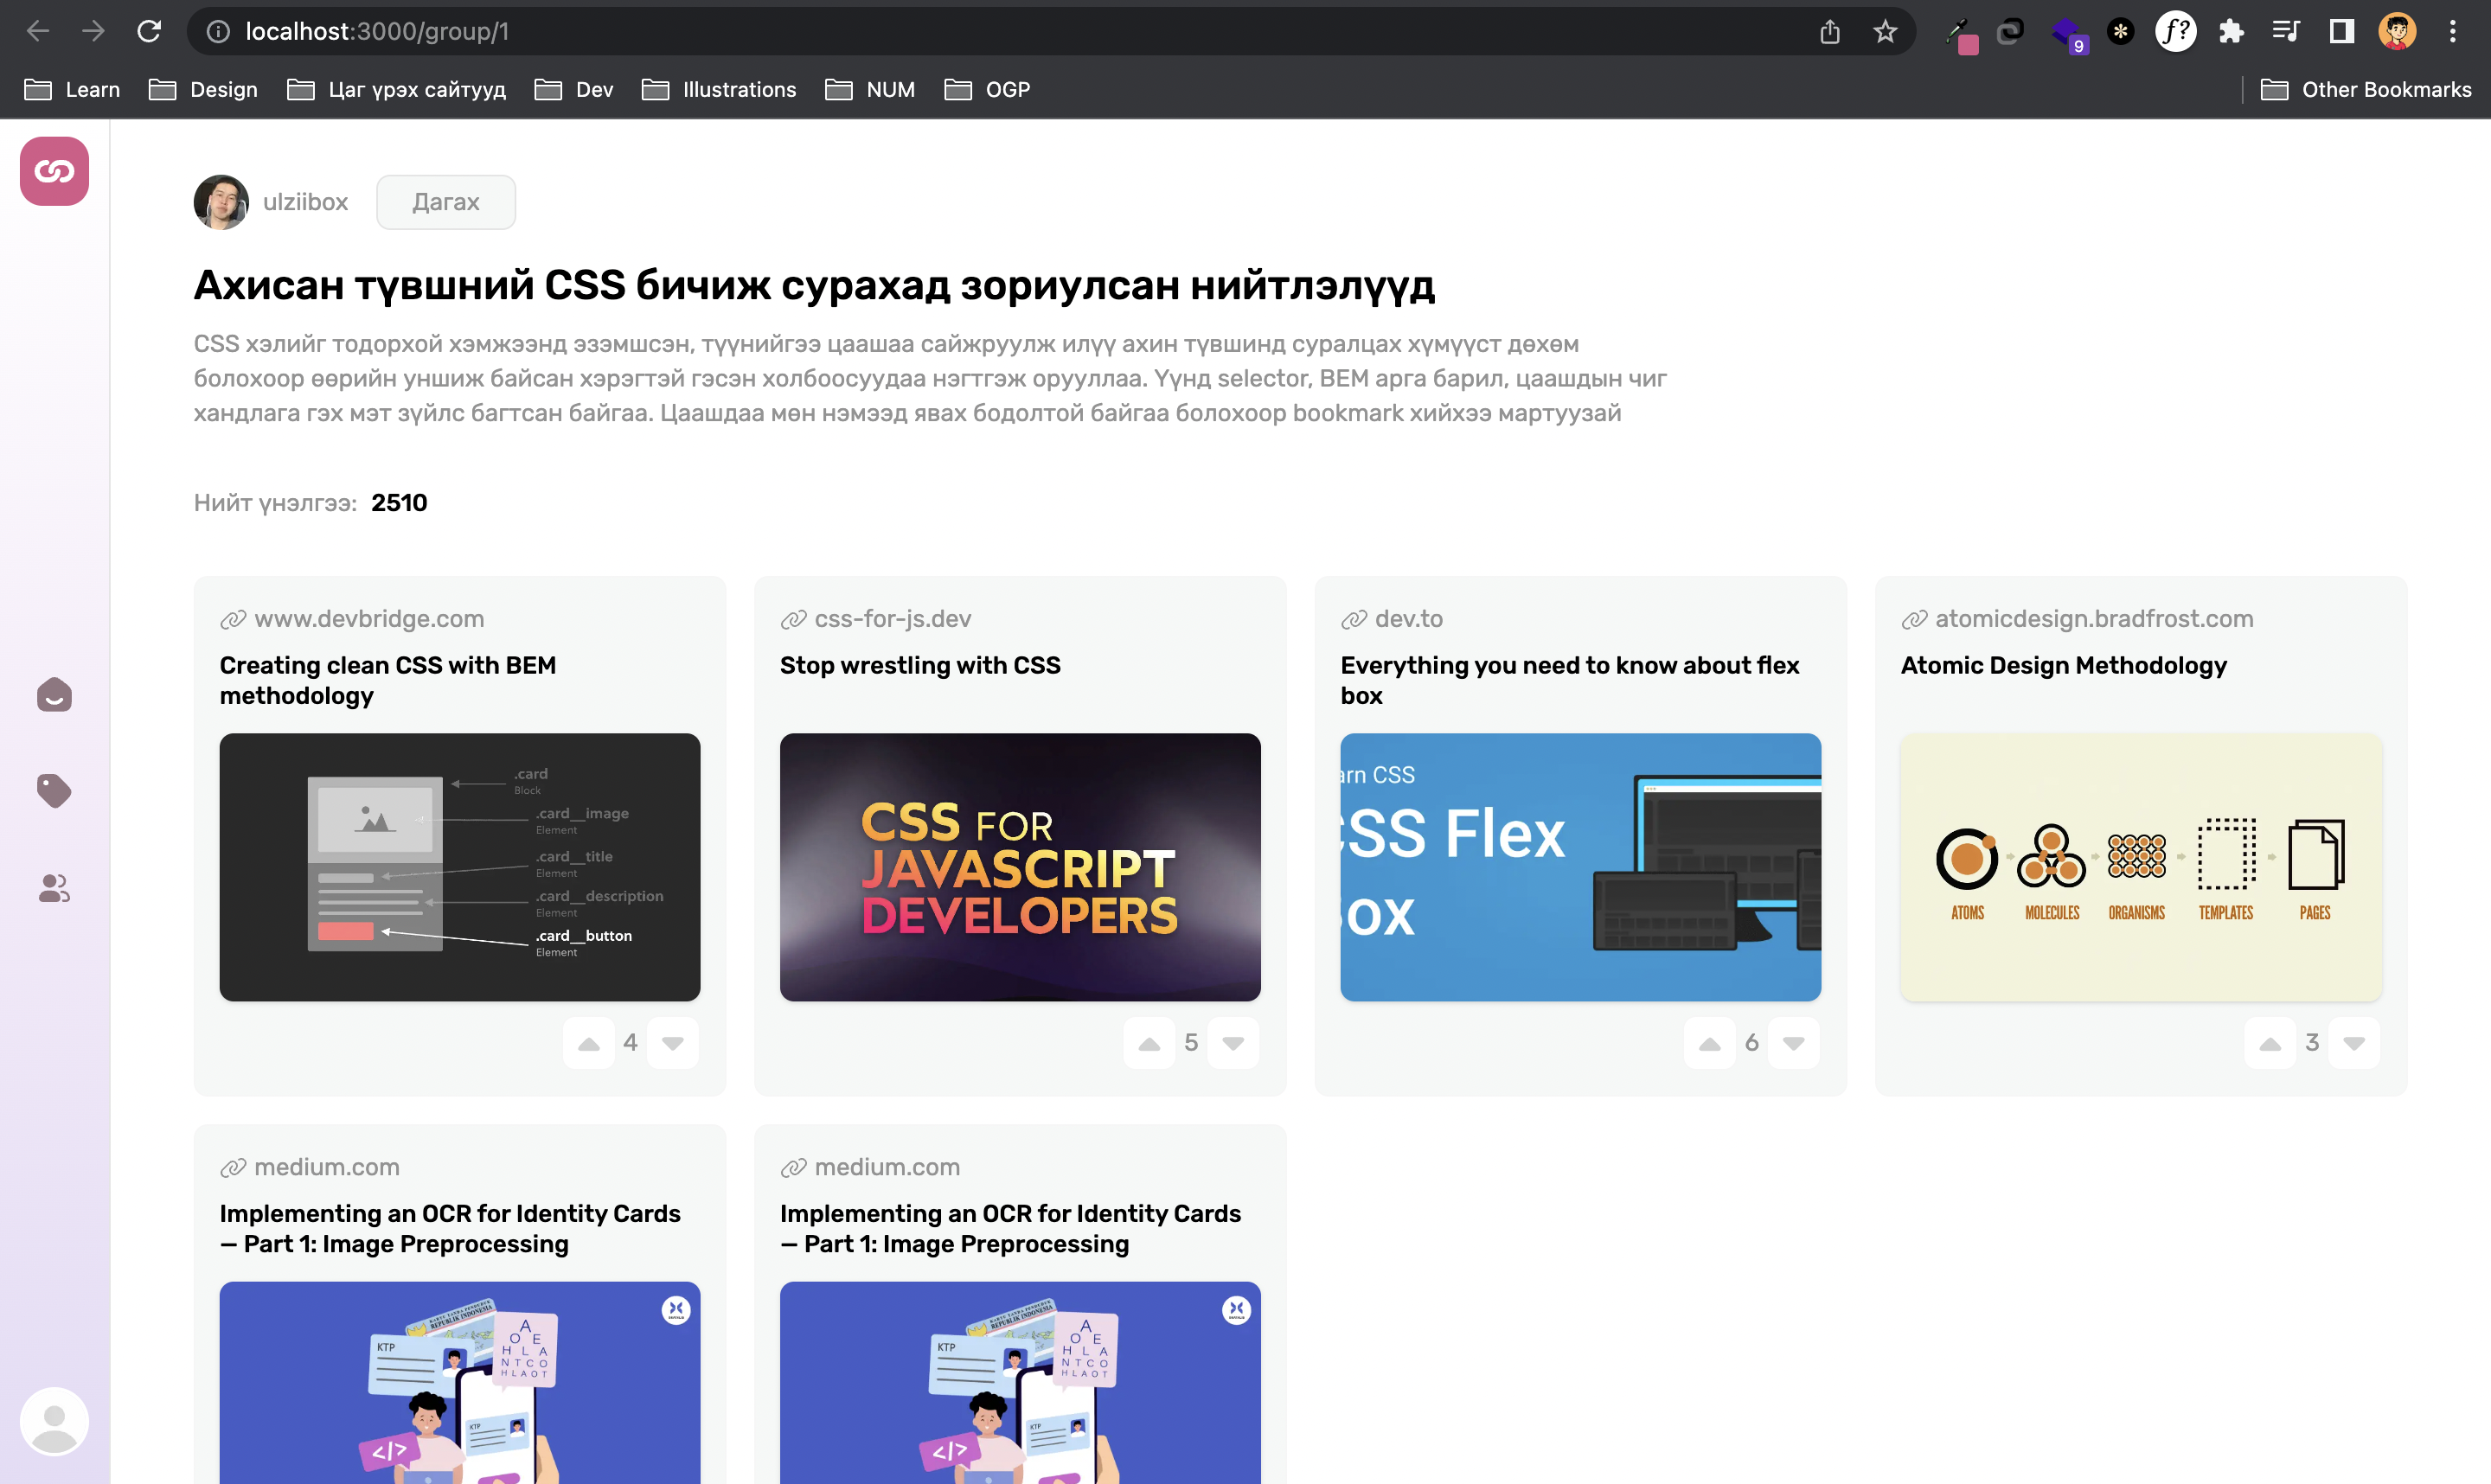
\includegraphics[width=13cm]{images/implement/group-link.png}
	\caption{Олон холбоосыг бүлэглэж харуулж буй хуудас}
	\label{fig:group-link}
\end{figure}

\begin{figure}[h]
	\centering
	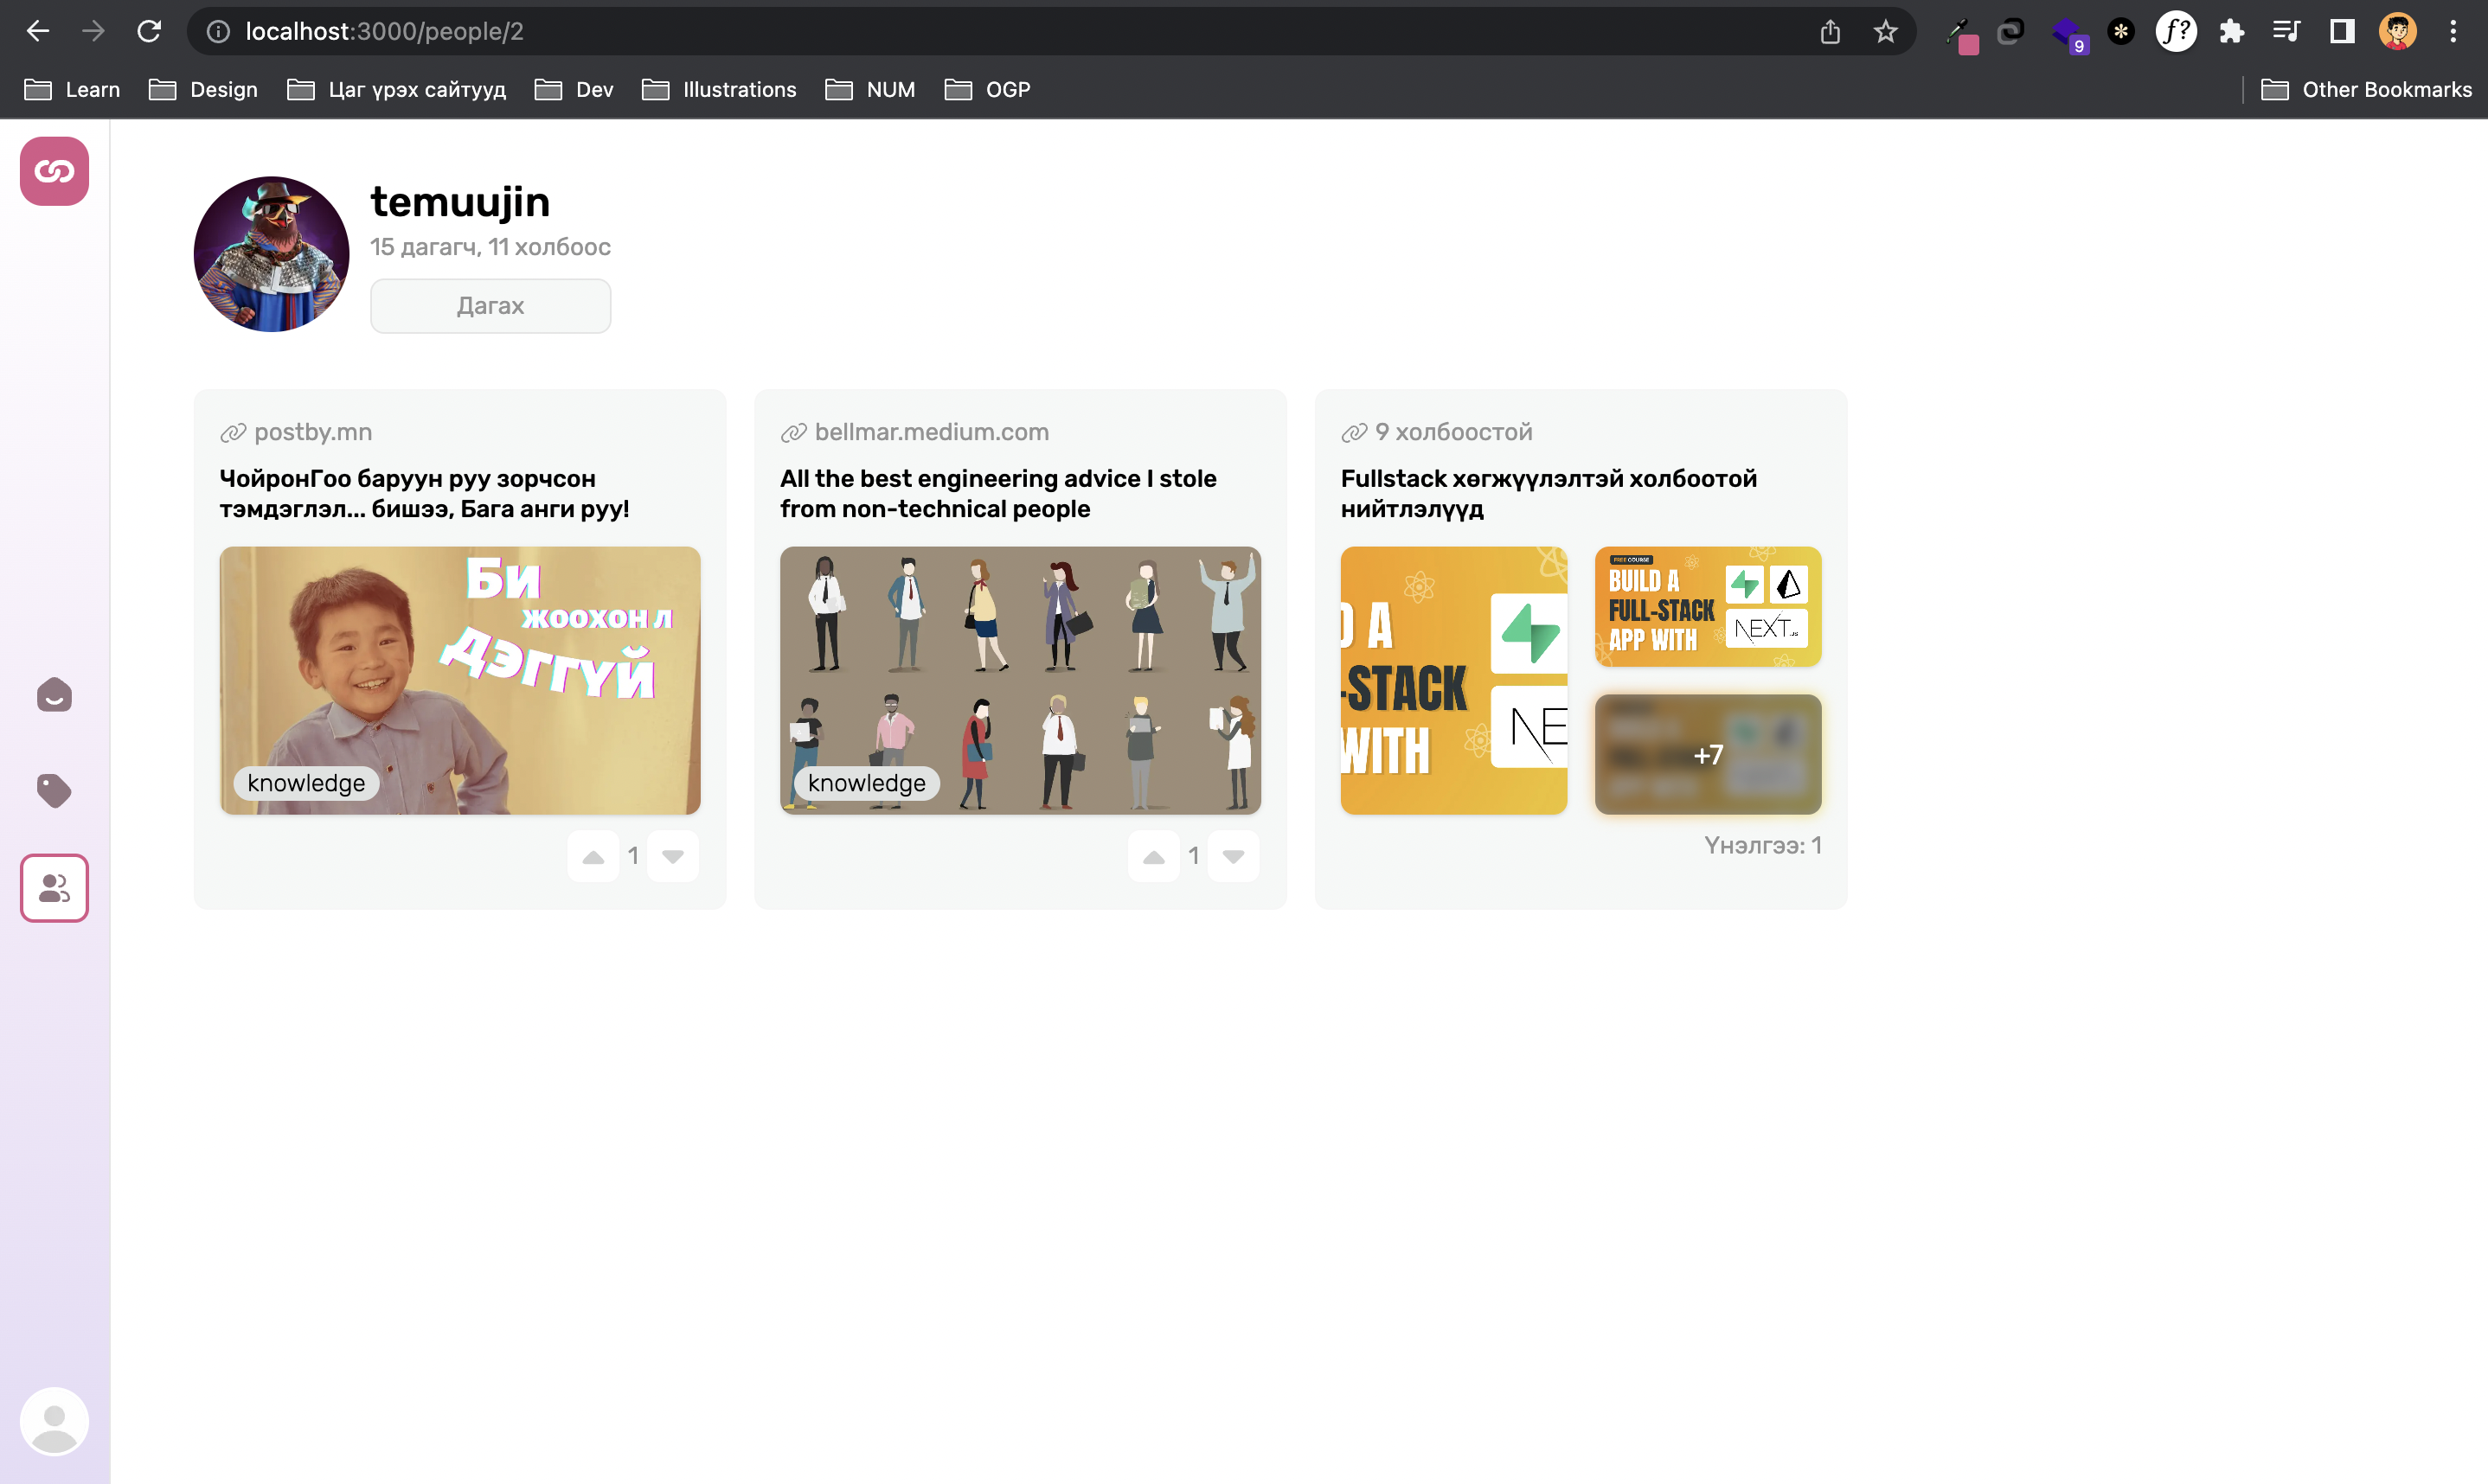
\includegraphics[width=13cm]{images/implement/user-posts.png}
	\caption{Сонгосон хэрэглэгчийн оруулсан холбоосуудыг нэг дор харах}
	\label{fig:user-posts}
\end{figure}
